\chapter{Preprocessing and Transformation}
\label{cha:preprocessing_transformation}

In order to pick out columns that have a significant impact on forecasting a movie's success, the following assumptions concerning the importance of information in the metadata were made:
\begin{itemize}
	\item The budget and revenue are crucial numbers.
	\item The release year has an impact on numbers such as budget and revenue.
	\item The genre, the production company and the runtime are important information.
\end{itemize}

In total, two datasets were used to create features for testing the different classifiers:
\textit{movies\_metadata.csv} and \textit{credits.csv}. The dataset \textit{movies\_metadata.csv} contains 45,463 rows and 24 columns. The dataset \textit{credits.csv} contains 45,463 rows and 3 columns. Since not all columns were needed as features for the data mining step, some columns were dropped. \textbf{Nicht gerade wisschenschaftlich hier} Figure \ref{img:mm_columns} gives an overview.

\begin{figure}
	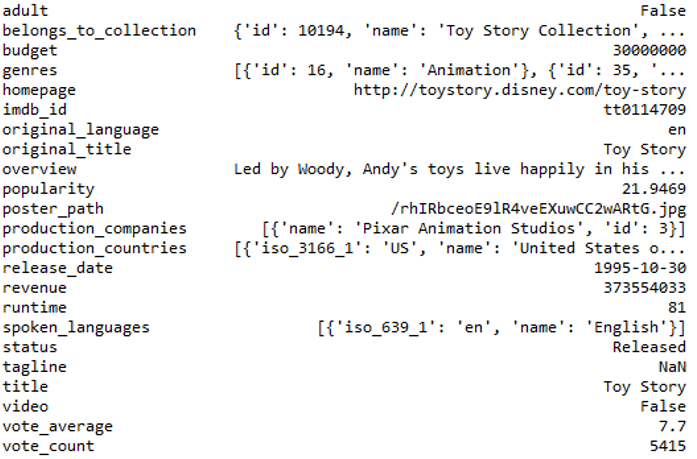
\includegraphics[width=\textwidth]{images/3_metadata_columns.png}
	\caption{Dropped columns of \textit{movies\_metadata.csv}}
	\label{img:mm_columns}
\end{figure}


In order to transform the data into a suitable representation for forecasting a movie's success, preprocessing was mandatory. All preprocessing steps included either the following:
\begin{itemize}
	\item Merging of columns
	\item binning of features
	\item extracting information out of columns
	\item one hot encoding
	\item normalizing
\end{itemize}

Before those steps could be applied, some columns were dropped out.

Display which ones here!

%can be considered to be in one of three different categories: Dropping columns, adding features and extracting and encoding information.

\begin{figure}
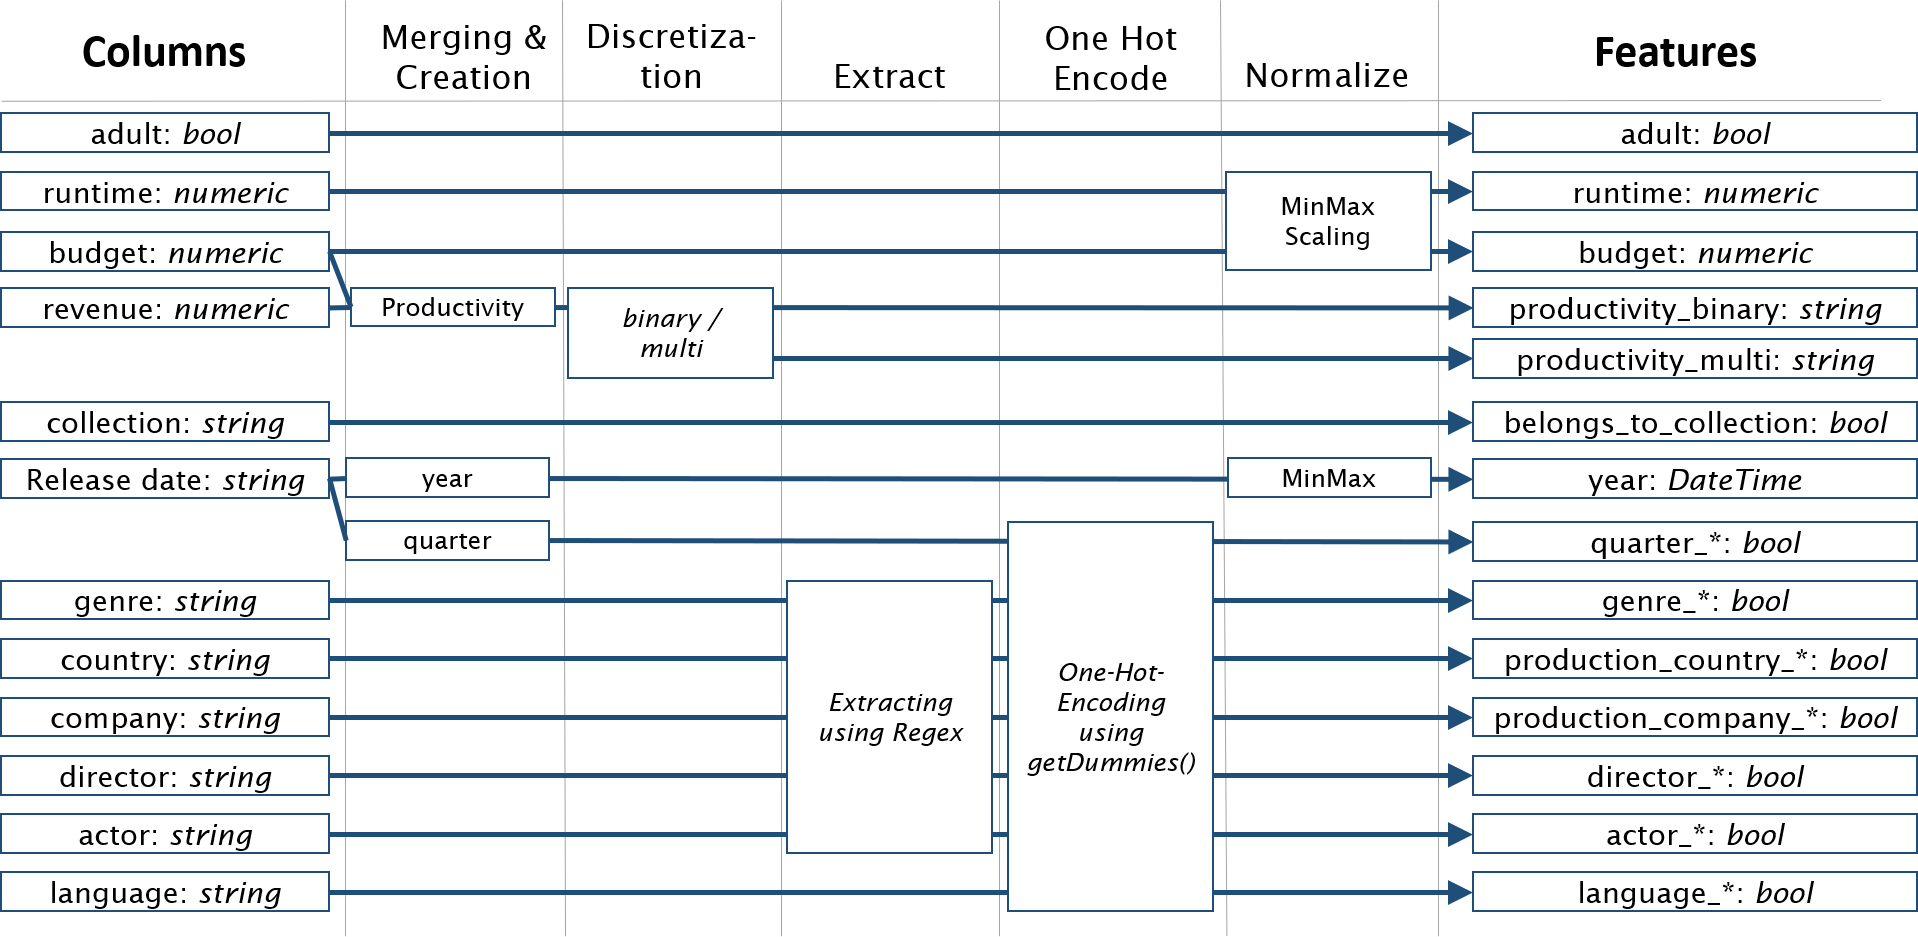
\includegraphics[width=\textwidth]{images/3_features.png}
\caption{Features created during preprocessing}
\label{img:features}
\end{figure}


\begin{itemize}
	\item Transform data into a representation that is suitable for the chosen data mining methods
	\begin{itemize}
		\item number of dimensions
		\item scales of attributes (nominal, ordinal, numeric)
		\item amount of data (determines hardware requirements)
	\end{itemize}
	\item Methods
	\begin{itemize}
		\item Aggregation, sampling
		\item Dimensionality reduction / feature subset selection
		\item Attribute transformation / text to term vector
		\item Discretization and binarization
	\end{itemize}
	\item Good data preparation is key to producing valid and reliable models
	\item Data preparation estimated to take 70-80\% of the time and effort of a data mining project!
\end{itemize}


\section{Preprocessing steps according to Python script}

\section{A list of problems we encountered}
\begin{enumerate}
	\item \textbf{list further problems we had and solved!}
	\item Prod. Comp.: Same prod. company named differently -> using Regex to solve (Steffen)
	\item dataset: 5 datasets have duplicates
\end{enumerate}
